% --- Module 2 ---

\chapter{Principal Component Analysis (PCA)}

\section{Empirical Covariance Matrices}

Before deriving PCA, it is useful to make explicit the role of the \emph{empirical covariance matrix}:
it is the object PCA works on directly.

\textbf{Setting.} We have $n$ observations $x_1, \dots, x_n \in \mathbb{R}^p$, i.e.\ $n$ individuals
on which we measure $p$ variables. We write $x_{ij}$ for the $j$-th variable of the $i$-th observation.

\dfn{Empirical mean}{
  The \emph{empirical mean} of the dataset is the vector
  \[
    \bar{x} = \frac{1}{n}\sum_{i=1}^{n} x_i =
    \begin{bmatrix} \bar{x}_1 \\ \bar{x}_2 \\ \vdots \\ \bar{x}_p \end{bmatrix} \in \mathbb{R}^p,
    \qquad \bar{x}_j = \frac{1}{n}\sum_{i=1}^{n} x_{ij}.
  \]
  Each component $\bar{x}_j$ is simply the mean of the $j$-th variable.
}

\dfn{Empirical covariance matrix}{
  The \emph{empirical covariance matrix} is
  \[
    S = \frac{1}{n}\sum_{i=1}^{n} (x_i - \bar{x})(x_i - \bar{x})^\top \in \mathbb{R}^{p \times p}.
  \]
  Entry by entry:
  \[
    S_{jk} = \frac{1}{n}\sum_{i=1}^{n} (x_{ij} - \bar{x}_j)(x_{ik} - \bar{x}_k).
  \]
}

\osservazione{
  Each term $(x_i - \bar{x})(x_i - \bar{x})^\top$ is a \emph{column $\times$ row} product
  ($p \times 1$ times $1 \times p$), hence a $p \times p$ matrix (of rank $1$).
  $S$ is the average of these $n$ matrices.
}

\osservazione{
  \textbf{$n$ or $n-1$?} Here we divide by $n$: this is the empirical-distribution convention
  (it coincides with the maximum-likelihood estimator in the Gaussian case).
  The usual \emph{unbiased} estimator divides by $n-1$ instead:
  \[
    S_{\text{unb}} = \frac{1}{n-1}\sum_{i=1}^{n} (x_i - \bar{x})(x_i - \bar{x})^\top = \frac{n}{n-1}\,S.
  \]
  For PCA \red{nothing changes}: the two matrices differ by a positive constant, so they have
  the same eigenvectors (the principal directions) and the same explained-variance ratios;
  only the numerical eigenvalues change, all multiplied by $\frac{n}{n-1}$.
}

\subsection{Matrix form}

\dfn{Data matrix}{
  The \emph{data matrix} $X \in \mathbb{R}^{n \times p}$ contains the observations \textbf{by row}:
  \[
    X = \begin{bmatrix} x_1^\top \\ \vdots \\ x_n^\top \end{bmatrix}
    \qquad \text{(rows = observations, columns = variables).}
  \]
  The data are \emph{centered} if $\bar{x} = 0_p$, i.e.\ every column of $X$ has zero mean.
}

\teorema{
  If the data are centered ($\bar{x} = 0_p$), then
  \[
    S = \frac{1}{n} X^\top X.
  \]
  In general, letting $X_c = X - \mathbf{1}_n \bar{x}^\top$ be the centered matrix
  ($\bar{x}^\top$ is subtracted from every row), we always have $S = \frac{1}{n} X_c^\top X_c$.
}

\pf{Proof}{
  The product $X^\top X$ can be written as a sum of column $\times$ row products:
  the $i$-th column of $X^\top$ is $x_i$ and the $i$-th row of $X$ is $x_i^\top$, so
  \[
    X^\top X = \sum_{i=1}^{n} x_i x_i^\top.
  \]
  If $\bar{x} = 0_p$, then $x_i - \bar{x} = x_i$ and the definition of $S$ becomes
  $S = \frac{1}{n}\sum_i x_i x_i^\top = \frac{1}{n}X^\top X$.
  In the general case, apply the same computation to $X_c$, whose rows are $(x_i - \bar{x})^\top$.
}

\osservazione{
  This is why in practice \textbf{data are always centered} before PCA: from then on
  the covariance is simply $\frac{1}{n}X^\top X$.
}

\subsection{How to read $S$}

The covariance matrix summarizes how the variables vary, individually and jointly:
\begin{itemize}
  \item \textbf{diagonal}: $S_{jj} = \frac{1}{n}\sum_i (x_{ij} - \bar{x}_j)^2$ is the \emph{variance}
        of variable $j$;
  \item \textbf{off-diagonal}: $S_{jk}$ is the \emph{covariance} between variables $j$ and $k$;
  \begin{itemize}
    \item $S_{jk} > 0$: when $j$ is above its mean, $k$ tends to be above its mean too;
    \item $S_{jk} < 0$: when one goes up, the other tends to go down;
    \item $S_{jk} \approx 0$: no \emph{linear} association.
  \end{itemize}
\end{itemize}

\esempio{
  If $p = 3$ (variables: height, weight, age):
  \[
    S = \begin{bmatrix}
      \mathrm{Var}(\text{height}) & \mathrm{Cov}(\text{height}, \text{weight}) & \mathrm{Cov}(\text{height}, \text{age}) \\
      \mathrm{Cov}(\text{weight}, \text{height}) & \mathrm{Var}(\text{weight}) & \mathrm{Cov}(\text{weight}, \text{age}) \\
      \mathrm{Cov}(\text{age}, \text{height}) & \mathrm{Cov}(\text{age}, \text{weight}) & \mathrm{Var}(\text{age})
    \end{bmatrix}.
  \]
}

\osservazione{
  The value of $S_{jk}$ depends on the units of measurement: a ``large'' covariance must be judged
  \emph{relative to the scales} of the variables. To compare, one uses the correlation
  \[
    r_{jk} = \frac{S_{jk}}{\sqrt{S_{jj}\,S_{kk}}} \in [-1, 1].
  \]
}

\subsection{Basic properties}

\mprop{Symmetry}{
  $S^\top = S$.
}

\pf{Proof}{
  Each term is symmetric: $\big((x_i - \bar{x})(x_i - \bar{x})^\top\big)^\top = (x_i - \bar{x})(x_i - \bar{x})^\top$,
  and a sum of symmetric matrices is symmetric.
}

\mprop{Positive semidefiniteness}{
  For every vector $a \in \mathbb{R}^p$,
  \[
    a^\top S a \geq 0.
  \]
  More precisely, $a^\top S a$ is the empirical variance of the data projected along $a$,
  i.e.\ of the numbers $a^\top x_1, \dots, a^\top x_n$.
}

\pf{Proof}{
  \[
    a^\top S a = \frac{1}{n}\sum_{i=1}^{n} a^\top (x_i - \bar{x})(x_i - \bar{x})^\top a
    = \frac{1}{n}\sum_{i=1}^{n} \big(a^\top x_i - a^\top \bar{x}\big)^2 \;\geq\; 0,
  \]
  since $a^\top (x_i - \bar{x})$ is a scalar, so it equals its transpose $(x_i - \bar{x})^\top a$.
  The last expression is exactly the empirical variance of the values $a^\top x_i$, whose mean is $a^\top \bar{x}$.
}

\cor{Nonnegative eigenvalues}{
  $S$ has $p$ real eigenvalues $\lambda_1 \geq \dots \geq \lambda_p \geq 0$ and an orthonormal basis
  of eigenvectors.
}

\pf{Proof}{
  Since $S$ is symmetric, the spectral theorem gives real eigenvalues and an orthonormal basis of eigenvectors.
  If $S v = \lambda v$ with $\|v\| = 1$, then by positive semidefiniteness
  \[
    \lambda = \lambda\, v^\top v = v^\top S v \geq 0. \qedhere
  \]
}

\osservazione{
  This is why positive semidefiniteness is crucial: eigenvalues of $S$ are \emph{variances}
  (along the eigenvector directions), so they cannot be negative.
  It is also the bridge to PCA: finding the direction $a$ (with $\|a\| = 1$) along which the data
  vary the most means maximizing $a^\top S a$.
}

\mprop{Rank bound}{
  If $X \in \mathbb{R}^{n \times p}$, then
  \[
    \operatorname{rank}(X^\top X) = \operatorname{rank}(X) \leq \min(p, n).
  \]
  For centered data, $S = \frac{1}{n}X_c^\top X_c$ satisfies the sharper bound
  \[
    \operatorname{rank}(S) \leq \min(p,\, n-1).
  \]
}

\pf{Proof}{
  \textbf{$\operatorname{rank}(X^\top X) = \operatorname{rank}(X)$.} We show $\ker(X^\top X) = \ker(X)$.
  If $Xv = 0$ then clearly $X^\top X v = 0$. Conversely, if $X^\top X v = 0$ then
  \[
    0 = v^\top X^\top X v = \|Xv\|^2 \quad\Longrightarrow\quad Xv = 0.
  \]
  Both matrices have $p$ columns, so by rank--nullity they have the same rank.
  And $\operatorname{rank}(X) \leq \min(p, n)$ because $X$ has $n$ rows and $p$ columns.

  \textbf{Centered case.} Centering imposes one linear constraint on the rows: they sum to zero,
  \[
    \sum_{i=1}^{n} (x_i - \bar{x}) = n\bar{x} - n\bar{x} = 0, \qquad\text{i.e.}\qquad \mathbf{1}_n^\top X_c = 0.
  \]
  So the $n$ rows of $X_c$ are linearly dependent and span a space of dimension at most $n-1$.
  Hence $\operatorname{rank}(S) = \operatorname{rank}(X_c) \leq \min(p, n-1)$ (the factor $\frac{1}{n}$ does not change the rank).
}

\osservazione{
  \textbf{High-dimensional setting.} When $n \ll p$ (few observations, many variables), the rank bound
  gives $\operatorname{rank}(S) \leq n-1 < p$: $S$ is \red{low rank}, hence singular, with at least
  $p - n + 1$ zero eigenvalues. This situation is called a \emph{high-dimensional setting} and
  requires special treatment.
}

\esempio{
  With $n = 2$ observations in $\mathbb{R}^3$, after centering $x_2 - \bar{x} = -(x_1 - \bar{x})$:
  all the data lie on a single line through $\bar{x}$, so $\operatorname{rank}(S) \leq 1$ even though $S$ is $3 \times 3$.
}

\section{Maximum Variance Principle}

The main objective of PCA is to find a \textbf{low-dimensional subspace} such that the
\textbf{projected data have maximum variance}. The idea:
\begin{itemize}
  \item if the projected points still \emph{spread out} substantially, the projection retains information;
  \item if the projected points \emph{collapse} into a small region, much structure has been removed.
\end{itemize}

From now on the data are \textbf{centered} ($\bar{x} = 0_p$) and $S = \frac{1}{n}X^\top X$.

\osservazione{
  \textbf{Notation clash.} The course uses $p$ both for the number of variables and for a direction
  vector. To keep them apart, here the direction is written in bold: $\bs{p} \in \mathbb{R}^p$.
}

\subsection{One direction}

\dfn{Latent score}{
  Given a direction $\bs{p} \in \mathbb{R}^p$, the \emph{latent score} of observation $i$ is
  \[
    z_i = \bs{p}^\top x_i \in \mathbb{R},
  \]
  i.e.\ the coordinate of $x_i$ along $\bs{p}$ (its projection, when $\|\bs{p}\| = 1$).
}

By the positive semidefiniteness proposition (the data are centered, so the scores have mean $0$),
the variance of the latent scores is
\[
  \operatorname{var}(z) = \frac{1}{n}\sum_{i=1}^{n} z_i^2 = \bs{p}^\top S \bs{p}.
\]

\osservazione{
  \textbf{Why the constraint $\bs{p}^\top\bs{p} = 1$.} Without it the problem has no finite maximum:
  for any scalar $c \in \mathbb{R}$,
  \[
    \operatorname{var}(cz) = (c\bs{p})^\top S (c\bs{p}) = c^2\, \bs{p}^\top S \bs{p},
  \]
  which, whenever $\bs{p}^\top S \bs{p} > 0$, becomes arbitrarily large by taking $|c|$ large.
  The constraint \red{fixes the scale}, so that we compare only \emph{directions}, not lengths.
}

\textit{Suggested exercises: 23 and 24.}

\dfn{PCA optimization problem (first direction)}{
  \[
    \max_{\bs{p} \in \mathbb{R}^p} \; \bs{p}^\top S \bs{p}
    \qquad \text{subject to} \qquad \bs{p}^\top \bs{p} = 1.
  \]
}

\teorema{
  Every stationary point of the problem satisfies the eigenvalue equation
  \[
    S\bs{p} = \lambda \bs{p},
  \]
  and at such a point the objective equals $\bs{p}^\top S \bs{p} = \lambda$. Therefore:
  \begin{itemize}
    \item the \textbf{principal directions} are (unit) \textbf{eigenvectors} of $S$;
    \item the \textbf{variance along each principal direction} is the corresponding \textbf{eigenvalue};
    \item the maximum is $\lambda_1$, the largest eigenvalue, attained at its eigenvector $\bs{p}_1$.
  \end{itemize}
}

\pf{Proof}{
  \textbf{Lagrange multiplier.} Consider
  \[
    \mathcal{L}(\bs{p}, \lambda) = \bs{p}^\top S \bs{p} - \lambda\,(\bs{p}^\top \bs{p} - 1).
  \]
  Since $S$ is symmetric, $\nabla_{\bs{p}}\, \bs{p}^\top S \bs{p} = 2S\bs{p}$ and $\nabla_{\bs{p}}\, \bs{p}^\top\bs{p} = 2\bs{p}$, so
  \[
    \nabla_{\bs{p}} \mathcal{L} = 2S\bs{p} - 2\lambda\bs{p} = 0 \quad\Longleftrightarrow\quad S\bs{p} = \lambda\bs{p}.
  \]
  Multiplying on the left by $\bs{p}^\top$ and using $\bs{p}^\top\bs{p} = 1$: $\bs{p}^\top S \bs{p} = \lambda$.
  Among the stationary points, the best one is the eigenvector with the largest eigenvalue.

  \textbf{Direct check that $\lambda_1$ is the maximum.} Write $S = P\Lambda P^\top$ (see below) and
  $\bs{y} = P^\top \bs{p}$; since $P$ is orthogonal, $\|\bs{y}\| = \|\bs{p}\| = 1$. Then
  \[
    \bs{p}^\top S \bs{p} = \bs{y}^\top \Lambda \bs{y} = \sum_{j=1}^{p} \lambda_j y_j^2
    \;\leq\; \lambda_1 \sum_{j=1}^{p} y_j^2 = \lambda_1,
  \]
  with equality for $\bs{y} = e_1$, i.e.\ $\bs{p} = \bs{p}_1$.
}

\textit{Suggested exercise: 25.}

\subsection{Spectral decomposition and $q$ directions}

\teorema{
  \textbf{(Spectral decomposition.)} Since $S$ is symmetric,
  \[
    S = P \Lambda P^\top,
  \]
  where
  \begin{itemize}
    \item $P = [\,\bs{p}_1 \mid \cdots \mid \bs{p}_p\,] \in \mathbb{R}^{p \times p}$ is orthogonal ($P^\top P = I$),
          its columns are the orthonormal eigenvectors $\bs{p}_j$;
    \item $\Lambda = \operatorname{diag}(\lambda_1, \dots, \lambda_p)$ contains the eigenvalues, ordered as
          \[
            \lambda_1 \geq \lambda_2 \geq \dots \geq \lambda_p \geq 0
          \]
          (nonnegative by the corollary on eigenvalues).
  \end{itemize}
}

To project onto a $q$-dimensional subspace ($q < p$) we take an orthonormal basis
$W = [\,\bs{w}_1 \mid \cdots \mid \bs{w}_q\,] \in \mathbb{R}^{p \times q}$, $W^\top W = I_q$. The variance
retained is the sum of the variances of the $q$ scores:
\[
  \sum_{k=1}^{q} \bs{w}_k^\top S \bs{w}_k = \operatorname{tr}(W^\top S W).
\]

\teorema{
  \textbf{(Best $q$-dimensional subspace.)} For every $W \in \mathbb{R}^{p \times q}$ with $W^\top W = I_q$,
  \[
    \operatorname{tr}(W^\top S W) \leq \lambda_1 + \dots + \lambda_q,
  \]
  with equality for $W = [\,\bs{p}_1 \mid \cdots \mid \bs{p}_q\,]$. Hence the best $q$-dimensional PCA
  subspace is \red{spanned by the eigenvectors of the $q$ largest eigenvalues}.
}

\pf{Proof}{
  Let $Y = P^\top W$ (still with orthonormal columns). Then
  \[
    \operatorname{tr}(W^\top S W) = \operatorname{tr}(Y^\top \Lambda Y) = \sum_{j=1}^{p} \lambda_j h_j,
    \qquad h_j = \sum_{k=1}^{q} Y_{jk}^2 .
  \]
  The weights satisfy $0 \leq h_j \leq 1$ ($h_j$ is the squared norm of the projection of $e_j$ onto
  the column space of $Y$) and $\sum_j h_j = \operatorname{tr}(Y^\top Y) = q$.
  With $q$ units of weight, each $\lambda_j$ receiving at most $1$, the sum $\sum_j \lambda_j h_j$ is
  largest by putting weight $1$ on the $q$ largest eigenvalues: $\sum_j \lambda_j h_j \leq \lambda_1 + \dots + \lambda_q$.
  For $W = [\,\bs{p}_1 \mid \cdots \mid \bs{p}_q\,]$ we get $h_1 = \dots = h_q = 1$, so equality holds.
}

\dfn{Captured and lost variance}{
  The variance \emph{captured} by the first $q$ principal components is
  \[
    V_q = \sum_{j=1}^{q} \lambda_j,
  \]
  and the variance \emph{lost} is
  \[
    J_{p-q} = \sum_{j=q+1}^{p} \lambda_j.
  \]
}

\osservazione{
  $V_q + J_{p-q} = \sum_{j=1}^{p} \lambda_j = \operatorname{tr}(S) = \sum_j S_{jj}$, the \emph{total variance}
  (sum of the variances of all variables). So the fraction of \textbf{explained variance} is
  \[
    \frac{V_q}{\operatorname{tr}(S)} = \frac{\lambda_1 + \dots + \lambda_q}{\lambda_1 + \dots + \lambda_p}.
  \]
  This ratio is unchanged if $S$ is rescaled (e.g.\ $n$ vs $n-1$).
}

\esempio{
  Suppose $p = 3$ and $S$ has eigenvalues $\lambda_1 = 5$, $\lambda_2 = 2$, $\lambda_3 = 1$, so $\operatorname{tr}(S) = 8$.
  \begin{itemize}
    \item $q = 1$: $V_1 = 5$, $J_2 = 3$, explained variance $5/8 = 62.5\%$;
    \item $q = 2$: $V_2 = 7$, $J_1 = 1$, explained variance $7/8 = 87.5\%$.
  \end{itemize}
  Projecting onto the plane spanned by $\bs{p}_1, \bs{p}_2$ loses only $12.5\%$ of the variance.
}

\section{A Worked Example in R}

We apply everything to a simulated dataset with $n = 150$ observations and $p = 2$ variables.

\begin{lstlisting}
set.seed(123)
n  <- 150
x1 <- rnorm(n, sd = 2)
x2 <- 0.6 * x1 + rnorm(n, sd = 0.5)   # x2 depends linearly on x1, plus noise
X  <- cbind(x1, x2)
\end{lstlisting}

\begin{figure}[H]
  \centering
  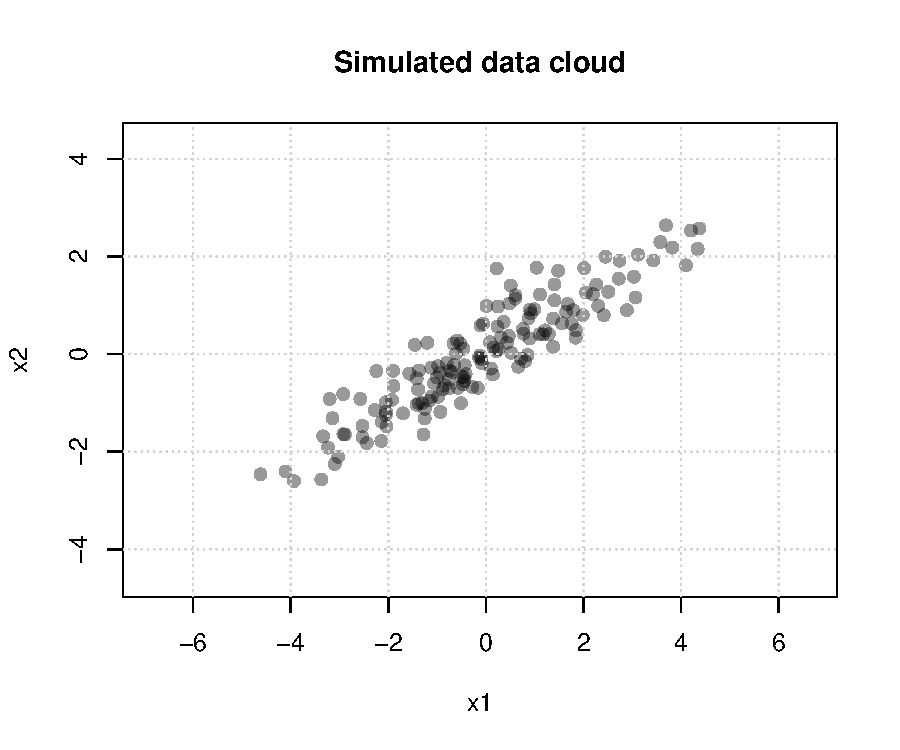
\includegraphics[width=0.6\textwidth]{img/pca-scatter.pdf}
  \caption{The simulated data cloud.}
\end{figure}

\subsection{Interpretation of the scatter plot}

This graph is the starting point. PCA is a \textbf{geometric} method, so we first look at the
\emph{shape} of the data cloud: if the cloud is \textbf{elongated}, most of the variation may lie close
to one direction. PCA formalizes that intuition.

\subsection{Covariance matrix and spectral decomposition}

We center the data and compute $S = \frac{1}{n}X_c^\top X_c$, then its eigen-decomposition:

\begin{lstlisting}
X_centered <- scale(X, center = TRUE, scale = FALSE)   # X_c: subtract column means
S <- crossprod(X_centered) / nrow(X_centered)          # crossprod(A) = t(A) %*% A

S
##          x1       x2
## x1 3.584051 2.004268
## x2 2.004268 1.334890

eig <- eigen(S)
eig$values
## [1] 4.757681 0.161260
eig$vectors
##            [,1]       [,2]
## [1,] -0.8629393  0.5053075
## [2,] -0.5053075 -0.8629393
\end{lstlisting}

\esempio{
  Reading the output with the theory:
  \begin{itemize}
    \item $S_{11} \approx 3.58$ and $S_{22} \approx 1.33$ are the variances; $S_{12} \approx 2.00 > 0$:
          $x_1$ and $x_2$ grow together (correlation $2.00/\sqrt{3.58 \cdot 1.33} \approx 0.92$);
    \item $\lambda_1 \approx 4.76$, $\lambda_2 \approx 0.16$: almost all variance is along $\bs{p}_1$;
    \item the columns of \texttt{eig\$vectors} are $\bs{p}_1, \bs{p}_2$: unit length and orthogonal;
    \item check: $\lambda_1 + \lambda_2 = 4.918941 = S_{11} + S_{22} = \operatorname{tr}(S)$.
  \end{itemize}
}

\osservazione{
  \textbf{Sign of eigenvectors.} If $\bs{p}$ is a unit eigenvector, so is $-\bs{p}$. Here R returns
  $\bs{p}_1 = (-0.86, -0.51)^\top$, but $(0.86, 0.51)^\top$ is equally valid. So principal directions
  and scores are defined only \emph{up to sign}.
}

\osservazione{
  \textbf{$n$ vs $n-1$ again.} Here $S$ uses denominator $n$. By contrast, \texttt{prcomp()} reports
  component variances with denominator $n-1$ (R's sample-covariance convention). This multiplies the
  eigenvalues by $n/(n-1)$ but does \red{not} change the principal directions, the latent scores
  (up to sign), the reconstructions or the explained-variance ratios.
}

\subsection{Principal directions}

We draw each principal direction as an arrow:

\begin{lstlisting}
mu     <- colMeans(X)
P      <- eig$vectors
lambda <- eig$values

arrows_df <- data.frame(
  x0 = mu[1], y0 = mu[2],
  x1 = mu[1] + 2 * sqrt(lambda[1]) * P[1, 1],
  y1 = mu[2] + 2 * sqrt(lambda[1]) * P[2, 1],
  x2 = mu[1] + 2 * sqrt(lambda[2]) * P[1, 2],
  y2 = mu[2] + 2 * sqrt(lambda[2]) * P[2, 2]
)
##             x0        y0        x1        y1        x2         y2
## x1 -0.04872574 0.0173874 -3.813231 -2.186977 0.3571088 -0.6756769
\end{lstlisting}

(then plotted with \texttt{ggplot2}: \texttt{geom\_point} for the data and one \texttt{geom\_segment}
with an arrow for each direction.)

\begin{figure}[H]
  \centering
  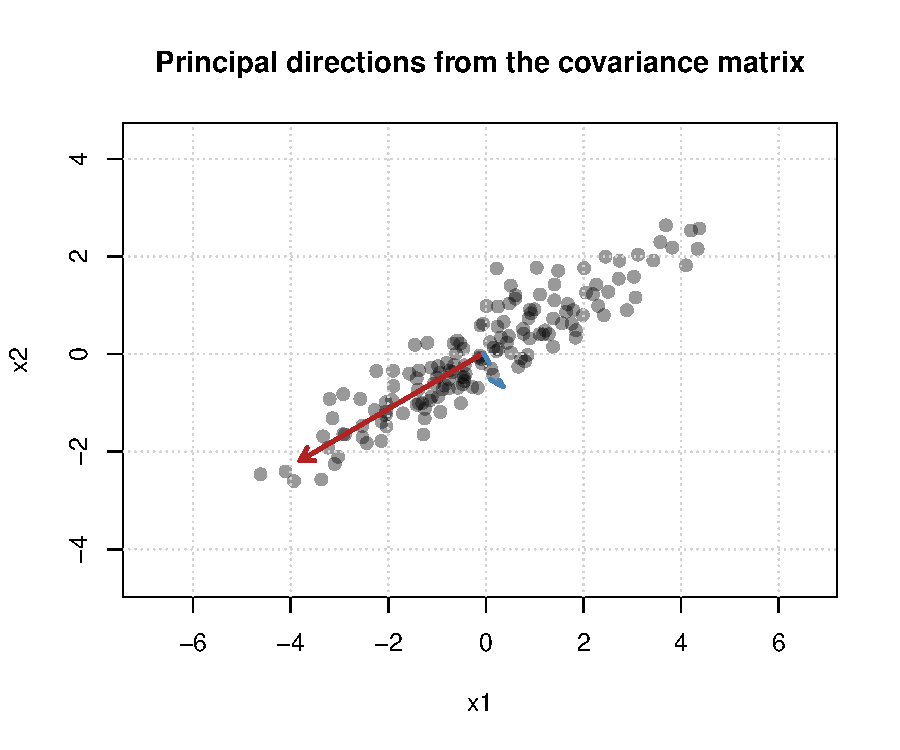
\includegraphics[width=0.6\textwidth]{img/pca-directions.pdf}
  \caption{First principal direction (solid, red) and second (dashed, blue).}
\end{figure}

\subsubsection{Interpretation}

Each arrow is
\[
  \underbrace{\mu}_{\text{start}} \;+\; \underbrace{2\sqrt{\lambda_j}}_{\text{length}} \; \underbrace{\bs{p}_j}_{\text{direction}},
  \qquad\text{i.e.\ in R:}\quad \texttt{mu + 2 * sqrt(lambda[j]) * P[, j]}.
\]
\begin{itemize}
  \item \textbf{start}: the empirical mean $\mu = \frac{1}{n}\sum_{i} x_i$, the center of the cloud;
        this is why both arrows start at \texttt{(mu[1], mu[2])};
  \item \textbf{direction}: the eigenvector, \texttt{P[, 1]} for the first principal direction and
        \texttt{P[, 2]} for the second;
  \item \textbf{length}: $\lambda_j$ is the \emph{variance} along $\bs{p}_j$, so $\sqrt{\lambda_j}$ is a
        \emph{standard deviation}, which has the same units as the data. The factor $2$ is only a
        visualization choice to make the arrows clearly visible.
\end{itemize}

\subsection{Explained variance ratio}

\begin{lstlisting}
prop_var <- eig$values / sum(eig$values)
\end{lstlisting}

\begin{center}
\begin{tabular}{ccc}
  \hline
  Component & Eigenvalue & Explained variance ratio \\
  \hline
  1 & 4.7577 & 0.9672 \\
  2 & 0.1613 & 0.0328 \\
  \hline
\end{tabular}
\end{center}

In this example \textbf{one component already explains $96.7\%$ of the variability}: with $q = 1$,
$V_1 = \lambda_1$ and the lost variance is only $J_1 = \lambda_2$.

\subsection{Projection and reconstruction}

With one retained component, each observation is projected onto the line through $\mu$ spanned by
the first principal direction.

\dfn{Score and reconstruction ($q = 1$)}{
  The \emph{score} of observation $i$ on the first component and its \emph{reconstruction} are
  \[
    z_i = \bs{p}_1^\top (x_i - \mu), \qquad
    \hat{x}_i = \mu + z_i\, \bs{p}_1 = \mu + \bs{p}_1 \bs{p}_1^\top (x_i - \mu).
  \]
  The \emph{reconstruction error} is the vector $x_i - \hat{x}_i$.
}

We compute this with \texttt{prcomp()}, where \texttt{\$x} are the scores $z_i$, \texttt{\$rotation} the
loadings (the matrix $P$) and \texttt{\$center} the mean $\mu$:

\begin{lstlisting}
pca_fit <- prcomp(X, center = TRUE, scale. = FALSE)

scores1   <- pca_fit$x[, 1, drop = FALSE]          # z_i         (n x 1)
loadings1 <- pca_fit$rotation[, 1, drop = FALSE]   # p_1         (2 x 1)

Xhat1 <- scores1 %*% t(loadings1)                  # z_i p_1^T   (n x 2)
Xhat1 <- sweep(Xhat1, 2, pca_fit$center, "+")      # add mu back to each row

head(data.frame(x1 = X[, 1], x2 = X[, 2],
                x1_hat = Xhat1[, 1], x2_hat = Xhat1[, 2]))
##           x1          x2      x1_hat      x2_hat
## 1 -1.1209513 -0.27870135 -0.97628325 -0.52575832
## 2 -0.4603550  0.10830813 -0.31560537 -0.13888812
## 3  3.1174166  2.03655127  3.18944333  1.91354762
## 4  0.1410168 -0.41957823 -0.09797001 -0.01144835
## 5  0.2585755  0.09541898  0.21413615  0.17131026
## 6  3.4301300  1.91788032  3.37056335  2.01960526
\end{lstlisting}

\begin{figure}[H]
  \centering
  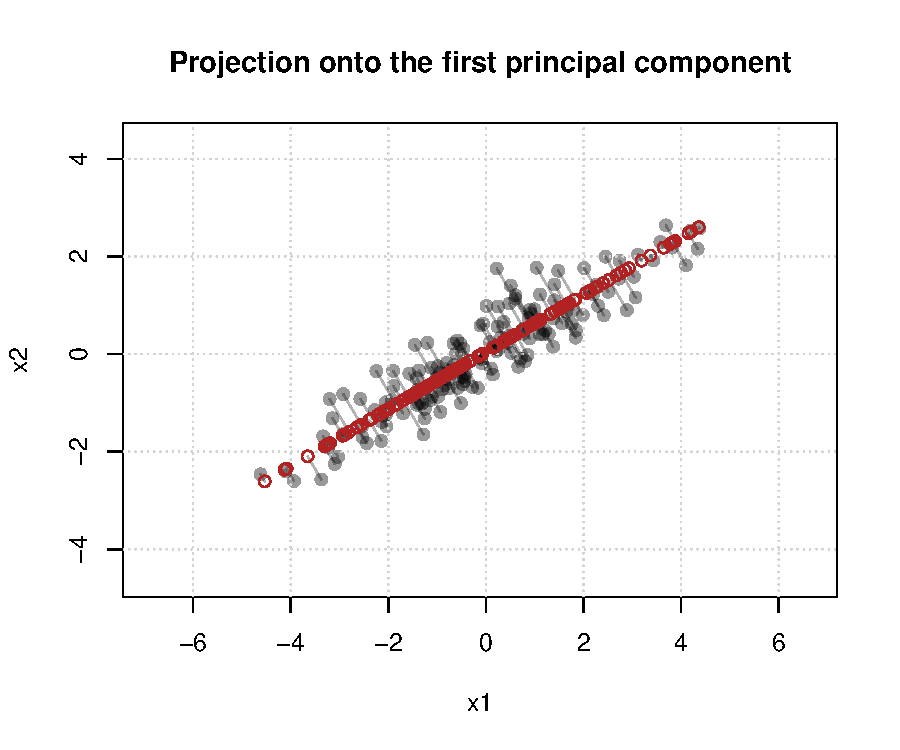
\includegraphics[width=0.6\textwidth]{img/pca-reconstruction.pdf}
  \caption{Original points (black), reconstructions $\hat{x}_i$ (red circles) and reconstruction errors (segments).}
\end{figure}

\subsubsection{Interpretation}

There are three geometric objects in this figure:
\begin{itemize}
  \item the \textbf{original data points} $x_i$ (\texttt{x1, x2});
  \item the \textbf{reconstructed points} $\hat{x}_i$ (\texttt{x1\_hat, x2\_hat}): the projections of the
        original observations onto the first principal component, so they all lie on one line;
  \item the \textbf{segments} between them, each representing the reconstruction error $x_i - \hat{x}_i$.
\end{itemize}
This is why the graph is useful: it shows visually what PCA does when only one component is kept.

\osservazione{
  The segments are \textbf{perpendicular} to the line: $x_i - \hat{x}_i$ is the component of $x_i - \mu$
  along $\bs{p}_2$. Hence the average squared length of the segments is exactly the lost variance:
  \[
    \frac{1}{n}\sum_{i=1}^{n} \|x_i - \hat{x}_i\|^2 = \lambda_2 = J_1 \approx 0.16.
  \]
  Maximizing the variance kept is the same as minimizing the reconstruction error.
}
